\documentclass[notes,11pt]{beamer}

%%%%%%%% tema e cor %%%%%%%%
\mode<presentation> {
\usetheme{Madrid}
}


\usepackage[english]{babel}
\usepackage[utf8]{inputenc}
\usepackage{graphicx} 
\usepackage{booktabs} 
\usepackage{listings}


\institute[] 
{
%================= logos no meio =====================
\vspace*{-0.35cm}

\includegraphics[width=1.8cm]{img/Diamond.eps}
\newline
\newline
% \texttt{gabryel.mason-williams@diamond.ac.uk\\dave.bond@diamond.ac.uk\\mark.basham@diamond.ac.uk}}
\texttt{\textsuperscript{1}Diamond Light Source \and \inst{2} University of Plymouth \and \inst{3} Rosalind Franklin Institute}
% \date{\today}
}
\AtBeginSection[]
{
\begin{frame}
\frametitle{Contents}
\tableofcontents[currentsection]
\end{frame}
}
%%%%%%%% Title %%%%%%%%
\title[Big Data]{High Performance Object Stores} 

% emails
%%%%%%%% Name %%%%%%%%
% \author[Gabryel Mason-Williams, Dave Bond, Mark Basham]{Gabryel Mason-Williams\\ Dave Bond\\ Mark Basham} 
\author[]{Gabryel Mason-Williams\textsuperscript{1,2} \and Dave Bond \inst{1} \and Mark Basham \inst{1,3}}
% \institute[shortinst]{\textsuperscript{1} Diamond Light Source \and \inst{2} University of Plymouth \and \inst{3} Rosalind Franklin Institute}

\begin{document}
\begin{frame}
\titlepage 

\end{frame}
\note{Hello I am Gabryel Mason-Williams, I study computer science at the university of Plymouth and have been working within Scientific Computing over the last 12 months. My supervisor is Dave Bond and co-supervisor is Mark Basham. }
\begin{frame}
\frametitle{Contents} 
\tableofcontents 
\end{frame}
\section{Part 1}
\section{Data at Diamond}
\begin{frame}{How is data generated}
    \centering
    \begin{figure}
        \centering
        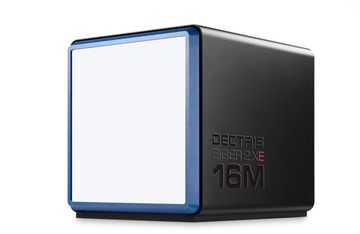
\includegraphics[width=\textwidth,height=0.45\textheight,keepaspectratio]{img/eiger2.jpg}
        \caption{Eiger Detector}
        \label{fig:my_label}
    \end{figure}
\end{frame}
\note{Diamond can be viewed as  giant video camera  filming a sample and it rotates on its axis. We do this using Fancy camera's known as detectors, now these camera's generate a incredible amount of unstructured data a second. Put to put the amount into perceptive, a Netflix movie your might stream for a evenings entertainment is about 7GB whereas our detectors are producing anywhere between 1GB/s to 40GB/s.}
\begin{frame}{Diamond = Netflix? }
\begin{columns}
    \begin{column}{0.30\textwidth}
    \begin{figure}
        \centering
        
\includegraphics[width=\textwidth,height=0.55\textheight,keepaspectratio]{img/Diamond.eps}
        \caption{Diamond}
        \label{fig:my_label}
    \end{figure}
    \end{column}
    \begin{column}{0.30\textwidth}
    \begin{figure}
        \centering
        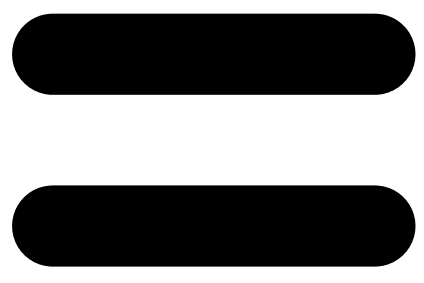
\includegraphics[width=\textwidth,height=0.55\textheight,keepaspectratio]{img/equals (2).png}
        \label{fig:my_label}
    \end{figure}
    \end{column}
    \begin{column}{0.30\textwidth}
    \begin{figure}
        \centering
        
\includegraphics[width=\textwidth,height=0.55\textheight,keepaspectratio]{img/netflix.jpg}
        \caption{Netflix}
        \label{fig:my_label}
    \end{figure}
    \end{column}
\end{columns}
\end{frame}
\note{At Diamond we stream science instead of movies}
\section{How do we store data \& The problems with it}
\begin{frame}{Computer Storage}
\begin{center}
    \Huge WHAT IS IT?
\end{center}{}
\end{frame}
\note{It is a way of handling and dealing with digital data, so you can retain it either temporally or permanently. There are different mechanises to do this currently at Diamond use a file storage}



\begin{frame}{Storage - File Storage}
\begin{columns}
    \begin{column}{0.47\textwidth}
    \begin{block}{File Storage}
        \begin{itemize}
            \item Hierarchical Structure 
            \item Files, Folders, Sub-directories, Directories
            \item Good with structured data 
            \item Filesystem
        \end{itemize}
    \end{block}
    \end{column}
    \begin{column}{0.47\textwidth}
        \begin{figure}
        \centering
        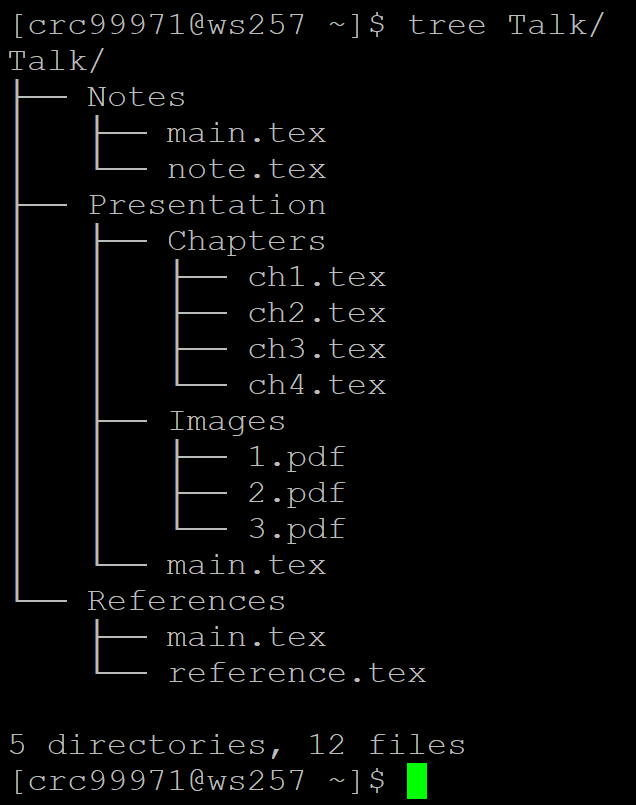
\includegraphics[width=\textwidth,height=0.7\textheight,keepaspectratio]{img/tree.PNG}
        \caption{File Storage}
        \label{fig:my_label}
    \end{figure}
    \end{column}
\end{columns}
\end{frame}
\note{So what about unstructured data, i.e images}
\begin{frame}{File Storage - Unstructured data}
    \begin{figure}
        \centering
        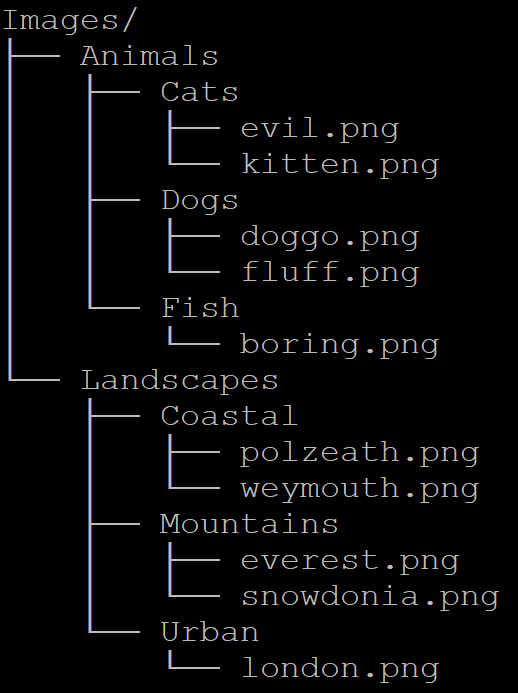
\includegraphics[width=\textwidth,height=0.7\textheight,keepaspectratio]{img/image-tree.png}
        \caption{Image Folder}
        \label{fig:my_label}
    \end{figure}  
\end{frame}


\begin{frame}{File Storage - Storing Images}
\begin{columns}
    \begin{column}{0.47\textwidth}
    \begin{figure}
        \centering
        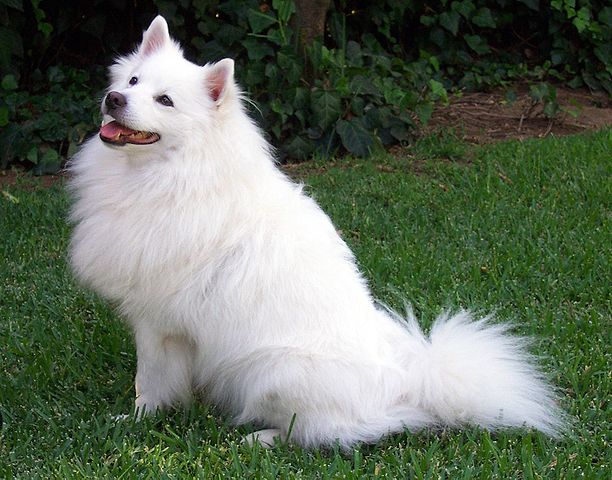
\includegraphics[width=\textwidth,height=0.45\textheight,keepaspectratio]{img/dog.jpg}
        \label{fig:my_label}
    \end{figure}
    \end{column}
    \begin{column}{0.47\textwidth}
    \begin{figure}
        \centering
        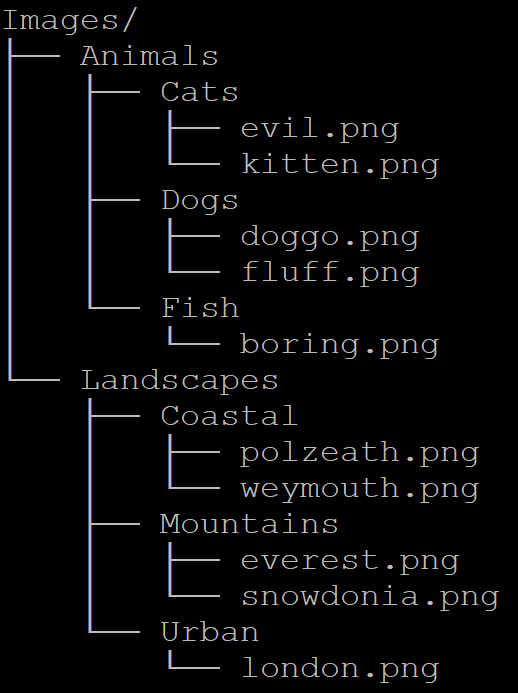
\includegraphics[width=\textwidth,height=0.55\textheight,keepaspectratio]{img/image-tree.png}
        \label{fig:my_label}
    \end{figure}
    \end{column}
\end{columns} 
\begin{block}{Where to store}
\begin{description}
    \item [A] Images/Animals/Dogs
    \item [B] Images/Animals/Cats
    \item [C] Images/Landscapes/Urban
\end{description}
\end{block}
\end{frame}
\note{If we have a file-system for storing images, that has subdirectories, Landscapes and Animals, and say Landscapes has subdirectories of Coastal, Mountain, Urban, etc. and Animals has subdirectories of; Fish, Dogs, Cats, etc. Now if we have well-defined images, of just Dogs, Coasts, Mountains and Cats. This system works perfectly well.}
\begin{frame}{File Storage - Storing Images}
\begin{columns}
    \begin{column}{0.47\textwidth}
    \begin{figure}
        \centering
        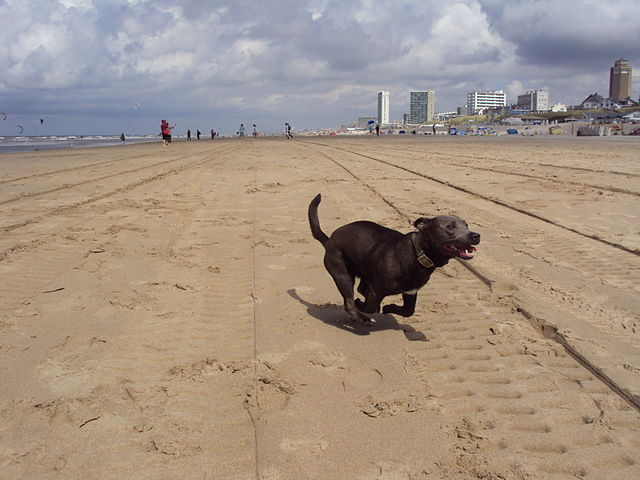
\includegraphics[width=\textwidth,height=0.45\textheight,keepaspectratio]{img/dog-or-beach.jpg}
        \label{fig:my_label}
    \end{figure}
    \end{column}
    \begin{column}{0.47\textwidth}
    \begin{figure}
        \centering
        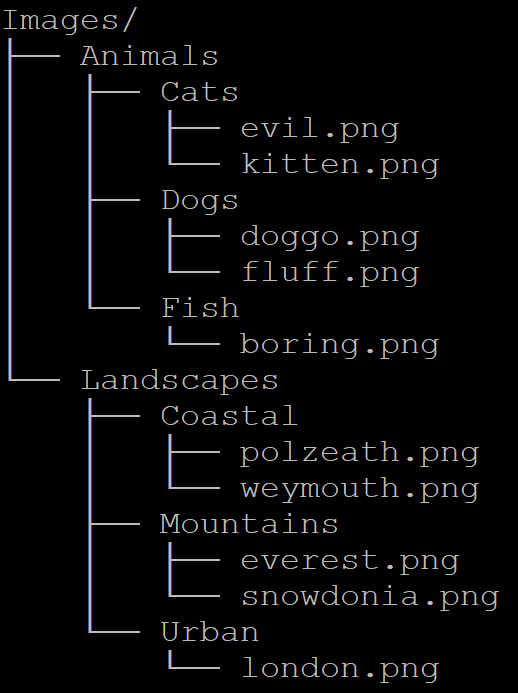
\includegraphics[width=\textwidth,height=0.55\textheight,keepaspectratio]{img/image-tree.png}
        \label{fig:my_label}
    \end{figure}
    \end{column}
\end{columns} 
\begin{block}{Where to store}
\begin{description}
    \item [A] Images/Animals/Dogs
    \item [B] Images/Landscapes/Coastal
    \item [C] Images/Landscapes/Urban
\end{description}
\end{block}
\end{frame}
\note{However, if we have an image of a Dog at the Beach, where do you place this image within this structure. It could either go in the Dogs or Coastal directory either would make sense. However, when looking for that image again, are you going to have remembered where you put it. Object Storage would make sense here as the data doesn't have an inherent structure as much as we can try.}


\begin{frame}{File Storage - Pros and Cons}
\begin{columns}[t]
    \begin{column}{0.47\textwidth}
    \begin{block}{Pros}
        \begin{itemize}
            \item Stores data in  Hierarchical structure
            \item Ideal for structured data
            \item Human interpretable 
            \item Already in use at Diamond
        \end{itemize}
    \end{block}
    \end{column}
    \begin{column}{0.47\textwidth}
    \begin{block}{Cons}
        \begin{itemize}
            \item Not good with unstructured data
            \item File size issues
            \item Lots of files
            \item Not cloud native
            \item Expensive
        \end{itemize}
    \end{block}
    \end{column}
\end{columns}
\end{frame}


\section{The solution maybe?}

\begin{frame}{Object Storage - What is it}
\begin{columns}
    \begin{column}{0.47\textwidth}
    \begin{block}{Object Storage}
        \begin{itemize}
            \item Archival data
            \item Stores data in  flat structure
            \item Performant with unstructured data
            \item Flexible data sizes, very small/very large
            \item RESTful API
        \end{itemize}
    \end{block}
    \end{column}
    \begin{column}{0.47\textwidth}
    \begin{figure}
        \centering
        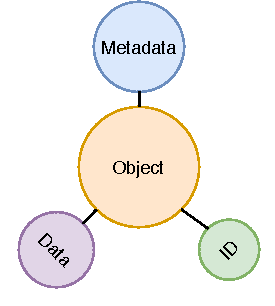
\includegraphics{img/object.pdf}
        \caption{Object Structure}
        \label{fig:my_label}
    \end{figure}
    \end{column}
\end{columns}
\end{frame}
\note{So this is a way to deal with unstructured data, in a sensible way that makes sense. Store the data as an object with a rich metadata that describes information about it, and associate an ID to it.}
\begin{frame}{Object Storage - Image Example}
    \begin{columns}
    \begin{column}{0.47\textwidth}
    \begin{figure}
        \centering
        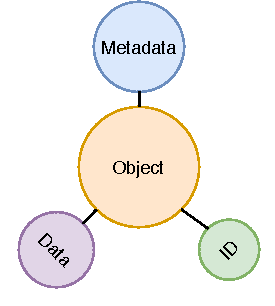
\includegraphics{img/object.pdf}
        \caption{Object}
        \label{fig:my_label}
    \end{figure}
    \end{column}
    \begin{column}{0.47\textwidth}
    \begin{figure}
        \centering
        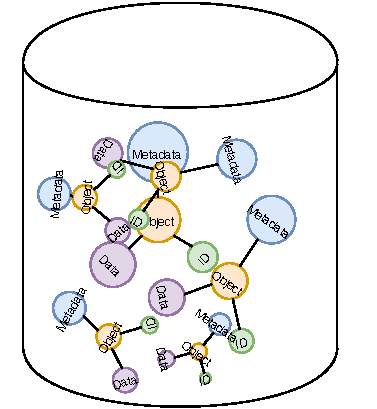
\includegraphics[width=\textwidth,height=0.55\textheight,keepaspectratio]{img/pool.pdf}
        \caption{Image Pool}
        \label{fig:my_label}
    \end{figure}
    \end{column}
\end{columns}
\end{frame}
\note{Instead, we can have a Pool called images and place the images inside that pool as objects, with metadata attached identifying what the image is instead.  Now we can just put images in the pool without having to worry where to put them. And when we want to get the image with a Dog at the Beach, we can look through the metadata and find images with that included that information. }

\begin{frame}{Object Storage - Pros and Cons}
\begin{columns}[t]
    \begin{column}{0.47\textwidth}
    \begin{block}{Pros}
        \begin{itemize}
            \item Flat structure
            \item Ideal for unstructured data
            \item Cloud native (RESTful API)
            \item Scales 
            \item Chunking
        \end{itemize}
    \end{block}
    \end{column}
    \begin{column}{0.47\textwidth}
    \begin{block}{Cons}
        \begin{itemize}
            \item Not as good with structured data
            \item Harder to browse and interact
            \item Editing data
        \end{itemize}
    \end{block}
    \end{column}
\end{columns}
\end{frame}
\note{So the flat structure makes the retrieval of data a lot easier and efficient, due to the way you access the data it is perfect for cloud integration. It scales easily with limited overhead, no servers dedicated to file structure. There are cons of course it is not a magic bullet to storage issues, most obvious is structure data, the fact it is not as easy to browse an object store and interact with it there are applications that help this problem however, DosNa being one, and you can't append to an object you need to read and write the whole thing.}
\section{What are we trying to solve}
\section{Part 2}
\begin{frame}{Part 2}
 \begin{block}{Catch up}
        \begin{itemize}
            \item Data at Diamond
            \item File Storage
            \item The problem with File Storage
            \item Object Storage and what it is
        \end{itemize}
    \end{block}
 \begin{block}{Where we are going}
 \begin{itemize}
     \item Ceph
     \item RAM
     \item Storage
 \end{itemize}
 \end{block}
\end{frame}
\section{Ceph}
\begin{frame}{Ceph - What is it}
\begin{figure}[h]
    \centering
    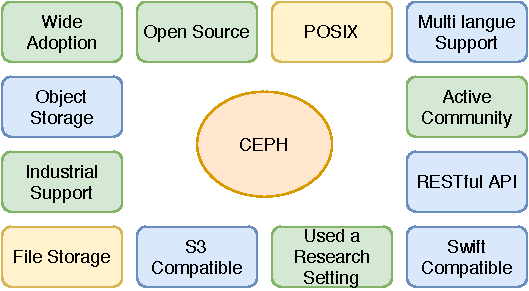
\includegraphics[width=\linewidth]{img/what-is-ceph.pdf}
\end{figure}
\end{frame}
\note{So Ceph is essence is Open Source scale-able distributed storage platform, that be used as a POSIX File System, Object store or Block device. It is S3 and Swift Compatible and has a a restful API that is implemented in multiple languages including Python,C++ and Java. It is approximately 14 years old and started as PhD project however has since been acquired by Redhat. It has many industrial and research facilities that use it, including STFC, CERN, OCADO and BLOOMBERG}
\begin{frame}{Ceph - Why is Diamond Interested}
\begin{block}{Reasons}
\begin{itemize}
        \item File \& Object Storage
        \item Open Source
        \item Scales
        \item Cloud integration
\end{itemize}
\end{block}
\end{frame}
\note{Now you make wonder why are interested in it for File storage when we deal with unstructured data, that because there is a lot of change that would be required some of which is already happening before we would go to full object store. }
\section{RAM}
\begin{frame}{RAM - What is it?}
\begin{columns}
    \begin{column}{0.47\textwidth}
    \begin{block}{RAM}
        \begin{itemize}
            \item Volatile 
            \item Fast
            \item Low latency
            \item Expensive
        \end{itemize}
    \end{block}
    \end{column}
    \begin{column}{0.47\textwidth}
        \begin{figure}
        \centering
        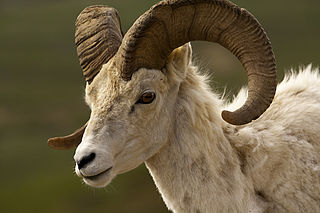
\includegraphics[width=\textwidth]{img/ram.jpg}
        \caption{Not this}
        \label{fig:my_label}
    \end{figure}
    \end{column}
\end{columns}
\end{frame}
\begin{frame}{RAM - Why we are interested}
    \begin{block}{Reasons}
        \item Transient data
        \item Fast
    \end{block}
\end{frame}
\note{When dealing with Transient data it shouldn't be stored in main memory if it can be avoided as this slows down the process.} 
\begin{frame}{RAM - How to access it?}
    \begin{block}{In a file system}
        \begin{itemize}
            \item Mount it in a directory
            \item Use a temporary file system, i.e tmpfs
            \item mount -t tmpfs -o size=8G tmpfs /mnt/ram
        \end{itemize}
    \end{block}
    \begin{block}{In object storage (Ceph)}
        \begin{itemize}
            \item Well its not as easy. 
        \end{itemize}
    \end{block}
\end{frame}
\note{It is quite simple, you would create a directory such as /mnt/ram and then apply a temporary file system to it. An wallah you have access to RAM in a file storage way.}

\section{Ceph and Storage Device}
\begin{frame}{Ceph - How to expose storage}
\begin{columns}
    \begin{column}{0.47\textwidth}
    \begin{block}{What the Computer sees}
    \begin{figure}
        \centering
        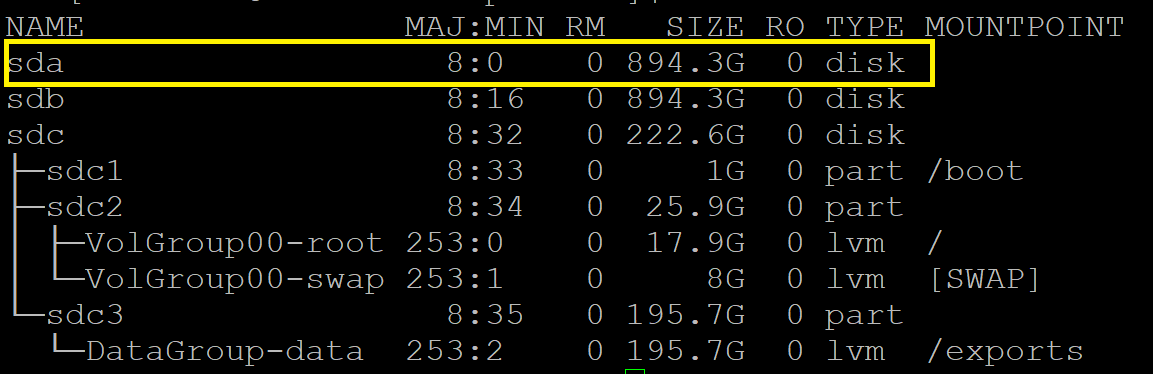
\includegraphics[width=\textwidth,height=0.55\textheight,keepaspectratio]{img/linuxdisk.PNG}
        \caption{Hard drive - sda}
        \label{fig:my_label}
    \end{figure}
    \end{block}
    \end{column}
    \begin{column}{0.47\textwidth}
    \begin{block}{What we see}
    \begin{figure}
        \centering
        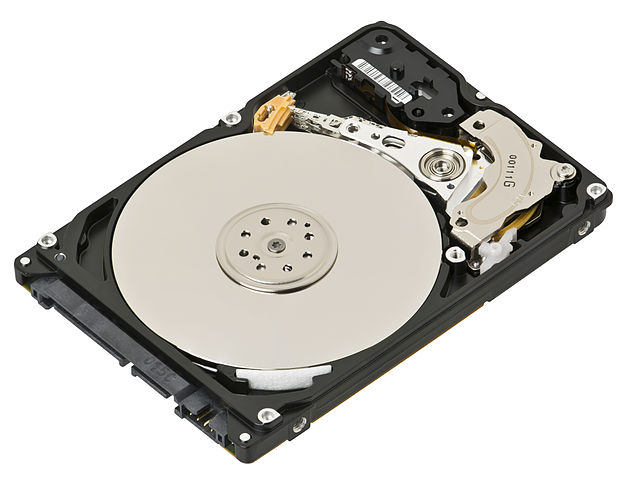
\includegraphics[width=\textwidth,height=0.55\textheight,keepaspectratio]{img/harddrive.jpg}
        \caption{Hard drive - sda}
        \label{fig:my_label}
    \end{figure}
    \end{block}
    \end{column}
\end{columns}
\end{frame}
\note{If we look here we can see that RAM is not exposed in the same way a hard drive is, this is an issue for us, as we want to be use RAM for storage} 

\begin{frame}{Can we make RAM = Disk?}
\begin{columns}
    \begin{column}{0.30\textwidth}
    \begin{figure}
        \centering
        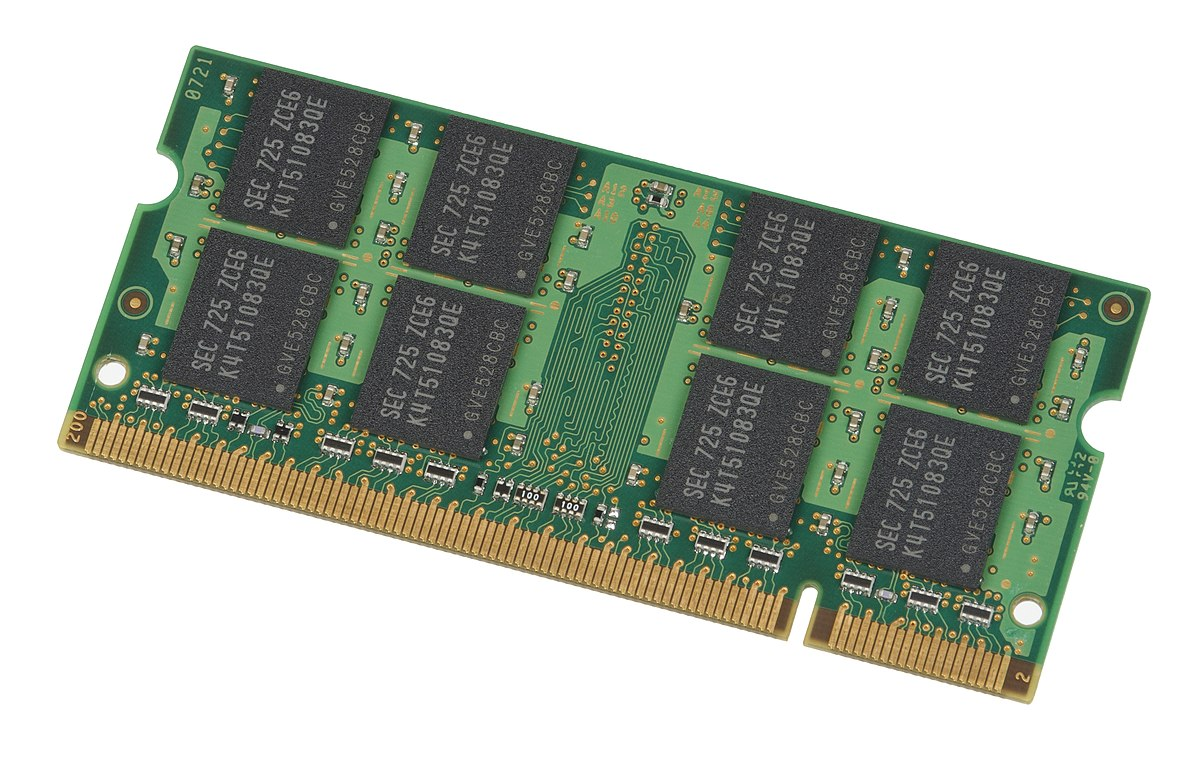
\includegraphics[width=\textwidth,height=0.55\textheight,keepaspectratio]{img/ramdrive.jpg}
        \caption{RAM Drive}
        \label{fig:my_label}
    \end{figure}
    \end{column}
    \begin{column}{0.30\textwidth}
    \begin{figure}
        \centering
        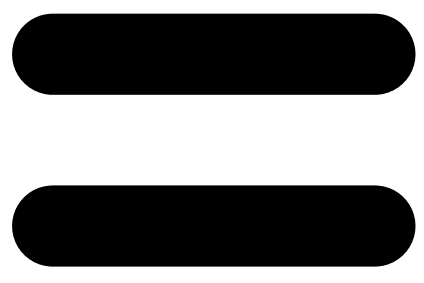
\includegraphics[width=\textwidth,height=0.55\textheight,keepaspectratio]{img/equals (2).png}
        \label{fig:my_label}
    \end{figure}
    \end{column}
    \begin{column}{0.30\textwidth}
    \begin{figure}
        \centering
        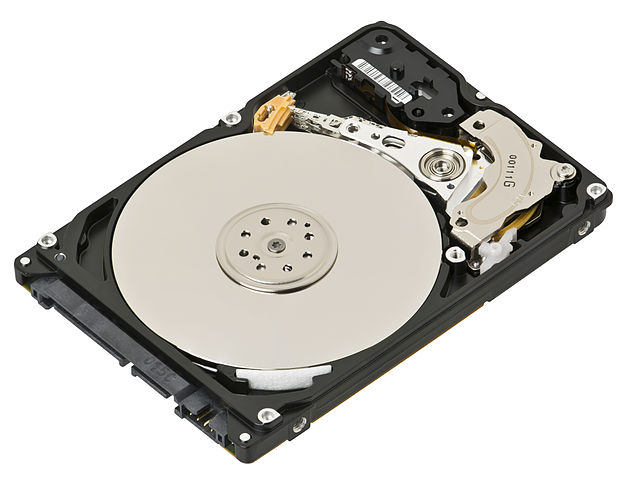
\includegraphics[width=\textwidth,height=0.55\textheight,keepaspectratio]{img/harddrive.jpg}
        \caption{Hard drive - sda}
        \label{fig:my_label}
    \end{figure}
    \end{column}
\end{columns}
\end{frame}
\note{Well the answer is yes and it isn't as difficult as it may seem, in essence we can trick the Linux kernel, into thinking that the RAM drive is actually a block device. How do we do this? Well there are two techniques, you can make your own Linux Module to do it or use the default, or change a pre-existing one to meet your needs.}
\begin{frame}{GRAM VS BRD}
    \begin{figure}
        \centering
        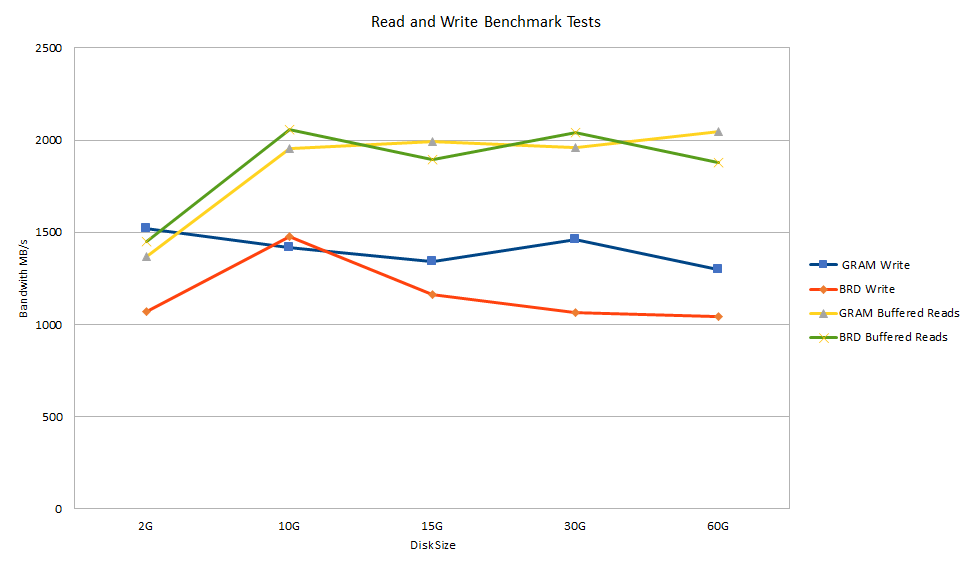
\includegraphics{img/gramVsbrd.png}
        \caption{RAM Block Devices}
        \label{fig:my_label}
    \end{figure}
\end{frame}
\note{So I should give a bit of background GRAM (General RAM) originally started off as my own kernel module, however the performance was to say for the least abysmal, i.e. the speed of a hard drive, due to the way I allocated memory and read and read from it. So after so serious googling I came across ZRAM (Which is a Compression RAM Block Device), so I removed the compression part and gave birth to GRAM. BRD is the default Linux provided block device, what is interesting to see is that BRD is less performant, that's a story for another day.}
\section{Part 3}
\begin{frame}{Part 2}
 \begin{block}{Catch up}
        \begin{itemize}
            \item What Ceph is 
            \item What Ram is
            \item How to access RAM
        \end{itemize}
    \end{block}
 \begin{block}{Where we are going}
 \begin{itemize}
    \item Distributed RAM Object Store
    \item Performance
    \item Use case
    \item Future Work and Conclusion
 \end{itemize}
 \end{block}
\end{frame}
\section{Compute Cluster}
\begin{frame}{Compute Cluster - What is it}
\begin{columns}
    \begin{column}{0.47\textwidth}
    \begin{block}{About}
        \begin{itemize}
            \item Interconnected Computers
            \item Disk less (No Storage/Hard drives)
            \item Lots of RAM
            \item Powerful CPUs \& GPUs
        \end{itemize}
    \end{block}
    \end{column}
    \begin{column}{0.47\textwidth}
        \begin{figure}
        \centering
        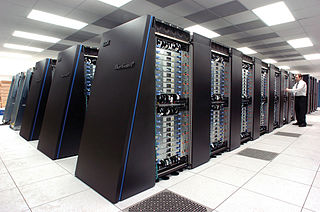
\includegraphics[width=\textwidth]{img/hpc.jpg}
        \caption{Actually this}
        \label{fig:my_label}
    \end{figure}
    \end{column}
\end{columns}
\end{frame}
\note{ I won't go into too much detail here as James will be giving a talk next week on this, however, what this means is that we have a system that has a lot of RAM that we can use as storage for running our Ceph instance}

\begin{frame}{Cluster - Deploying Ceph}
 \begin{figure}
     \centering
     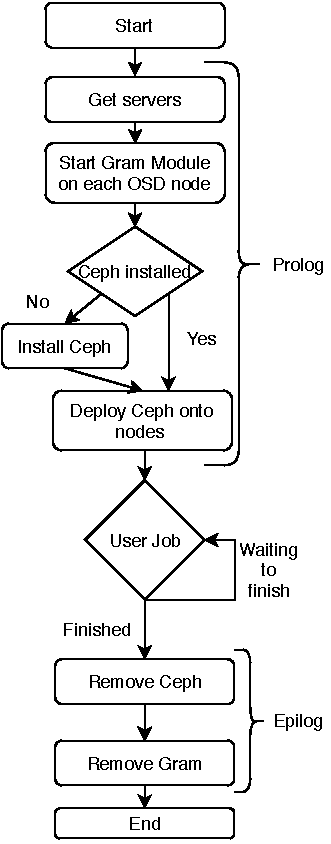
\includegraphics[width=\textwidth,height=0.7\textheight,keepaspectratio]{img/UGECeph.pdf}
     \caption{Deploy Script}
     \label{fig:my_label}
 \end{figure}
\end{frame}
\note{Walk through Script}
\section{Performance}
\begin{frame}{Performance - What we got}
    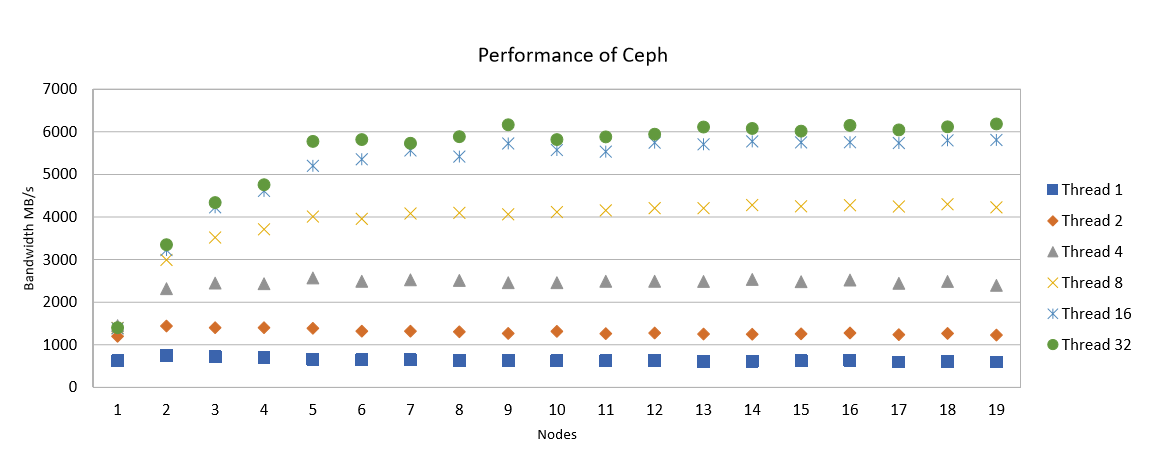
\includegraphics[width=\textwidth]{img/scale.PNG}
\end{frame}
\note{So the network limit is approximately 6GB/s, so we are able to reach this in 6 Nodes, which is very good to see, if run on a compute cluster with more per format RAM we could potentially see this number be a lot lower, as this cluster operates at approx 1GB/s per OSDs. Whats interesting to see here is that 16 threads should do the job just fine which means we can run a job at the same time creating a hyper-converged platform.}
\section{Use cases}
\begin{frame}{Distributed Ram Object Store - Use Case}
    \begin{columns}
    \begin{column}{0.47\textwidth}
    \begin{block}{Tomography data}
        \begin{itemize}
            \item Savu
            \item Has an object store plugin DosNa
            \item See objects and data processing in real time
            \item Run irrespective of current File system performance 
        \end{itemize}
    \end{block}
    \end{column}
    \begin{column}{0.47\textwidth}
    \begin{figure}
        \centering
        \includegraphics[width=\textwidth,height=0.45\textheight,keepaspectratio]{img/savu.PNG}
        \label{fig:my_label}
    \end{figure}
    \end{column}
\end{columns}
\end{frame}

\begin{frame}{High Performance Object Store - Use Case }
\begin{block}{MX Pipeline}
        \begin{itemize}
            \item Remove file system issues
        \end{itemize}
    \end{block}
\end{frame}
\section{Conclusion}
\begin{frame}{Conclusion \& Future Work}
    \begin{center}
        \Huge Conclusion \& Future Work
    \end{center}
\end{frame}
\section{Questions}
\begin{frame}{Questions}
\begin{center}
    Thanks for listening any questions?    
\end{center}{}
\begin{center}
    Contact details:
    \\
        Slack: @Gabryel (Gabryel Mason-Williams)
    \\
        Email: gabryel.mason-williams@diamond.ac.uk 
\end{center}{}
\end{frame}
\note{I would like to say thank you to my supervisors Dave Bond, Mark Basham, scientific computing, the ceph community and everyone who's compute time I took whilst running my tests}


\end{document}